\documentclass[tikz, border=5pt]{standalone}
\usepackage{tikz}
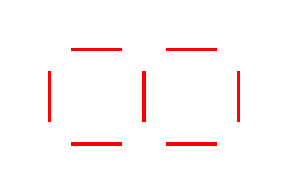
\begin{tikzpicture}[>=stealth, node distance=1.2cm]
    \tikzstyle{format} = [draw, very thick, circle, minimum size=5.0mm, inner sep=0pt]

    \begin{scope}
        \path[-, very thick]
          node[white, format] (A1) {$A_1$}
          node[white, format, right of=A1] (A2) {$A_2$}
          node[white, format, right of=A2] (A3) {$A_3$}
          node[white, format, below of=A1] (A4) {$A_4$}
          node[white, format, right of=A4] (A5) {$A_5$}
          node[white, format, right of=A5] (A6) {$A_6$}
          
          (A1) edge[red] (A2)
          (A1) edge[red] (A4)
          (A2) edge[red] (A3)
          (A4) edge[red] (A5)
          (A5) edge[red] (A6)
          (A2) edge[red] (A5)
          (A3) edge[red] (A6);
    \end{scope}
\end{tikzpicture}